%%-------------------------------------------------------------------------------------------------
%%                           Template Notes:
%% Make sure to have all template files from klmweb/revisions/templates/JJH_Beamer before using
%% this file. Also please read the Beamer Reference document for typists if you have any questions
%% on the usage of this template.
% -------------------------------------------------------------------------------------------------
\documentclass[dynamic]{JJH-Beamer}

%% -- Extra Packages (Place Packages here if they are not included in the default template)--------

\usepackage{adjustbox}
\usepackage{booktabs}
\usepackage{soul}
\usepackage{tabularx}
\usepackage{graphicx}
\usepackage{colortbl}
\usepackage[para]{threeparttable}
\usepackage{epstopdf}
\usepackage{subfig}
\usepackage{bbding}
\usepackage{appendixnumberbeamer}
\usepackage{rotating}
\usepackage{geometry}
\usepackage{pdflscape}

%% ------ Extra Preamble Definitions (Place any other extra preamble stuff here) ------------------

\newcommand{\mr}{\multirow}
\newcommand{\mc}{\multicolumn}
\newcolumntype{L}[1]{>{\raggedright\let\newline\\\arraybackslash\hspace{0pt}}m{#1}}
\newcolumntype{C}[1]{>{\centering\let\newline\\\arraybackslash\hspace{0pt}}m{#1}}
\newcolumntype{R}[1]{>{\raggedleft\let\newline\\\arraybackslash\hspace{0pt}}m{#1}}

\newcommand{\backupbegin}{
   \newcounter{finalframe}
   \setcounter{finalframe}{\value{framenumber}}
}
\newcommand{\backupend}{
   \setcounter{framenumber}{\value{finalframe}}
}

\newcommand*\leftright[2]{%
  \leavevmode
  \rlap{#1}%
  \hspace{0.5\linewidth}%
  #2}
% ------------ Title, author, date (ALWAYS UPDATE THESE THINGS) -----------------------------------

\def \thetitle {Summary of the Reggio Evaluation} % Full title goes here

\def \theshorttitle {Reggio} %Short title goes here

\def \theauthor {Reggio Team} % Author name(s) go here

\def \theshortauthor {Reggio Team} % Short author name(s) go here; should fit on this one line.

\def \thedate {December 20th, 2016} % Date and venue information

\def \eventnotes {\noindent
\textbf{Date:} Tuesday, December 20th, 2016 \\
\textbf{Event Title:} Call with the Jacobs Foundation \\
\textbf{Location:}  \\
\textbf{Presentation Title:} Summary of the Reggio Evaluation
} % Other event info, to appear on the front of the private notes

% -------------------------------------------------------------------------------------------------

\begin{document}
%\renewcommand*{\inserttotalframenumber}{\pageref{lastframe}}

\mode<all>{\theTitlePages} % Macro to insert both title pages DO NOT REMOVE!

%%
%% ------------------------- Content starts here --------------------------------------------------
\begin{frame}
\frametitle{Overview}
\begin{itemize}
\item This handout summarizes the process and findings of our evaluation of the Reggio Approach
\item Empirical results do not emphatically support that the Reggio Approach has strong effects
\begin{itemize}
	\item Positive results are found in the adult cohorts when compared to other adults who did not attend preschool
	\item The Reggio Approach improves some non-cognitive and mental health outcomes for children and adolescents
\end{itemize}
\item Historical evidence collected by CEHD indicates that alternative preschools were available and regulated leading to quality alternatives
\item We also outline issues with the design of the study and data collection 
\end{itemize}

\end{frame}

% -------------------------------------------------------------------------------------------------

\begin{frame}
\frametitle{Discussion}
\begin{itemize}
	\item Historical context
	\begin{itemize}
		\item Unpublished historical evidence and empirical results indicate that alternatives were available that had positive effects on children
		\item Paper records indicate that take-up of these programs was very high in Reggio Emilia and Padova
		\item Results from our survey indicate that even though the specific combination of components is unique to the Reggio Approach, an increasing number of these components were adopted by other programs over time
	\end{itemize}
	\item Data limitations
	\begin{itemize}
		\item More family characteristics, especially for the adult cohorts, would help better model the effect of the Reggio Approach by accounting for family disadvantage more fully
		\item Some issues in data collection limit some of the key outcomes such as IQ, school grades, and income
	\end{itemize}
\end{itemize}
\end{frame}


% -------------------------------------------------------------------------------------------------

\begin{frame}
\frametitle{Sample}
\begin{itemize}
	\item Five age cohorts chosen to capture short-, medium-, and long-term effects and different levels of exposure to the Reggio Approach
	\begin{itemize}
		\item Children (b. 2006)
		\item Adolescents (b. 1994)
		\item Adults in their 30s (b. 1980-1981)
		\item Adults in their 40s (b. 1969-1970)
		\item Adults in their 50s (b. 1954-1959)
	\end{itemize}
	\item Individuals sampled if they were living in the same city as they did when they were of preschool age
		\begin{itemize}
			\item Reggio Emilia
			\item Parma
			\item Padova
		\end{itemize}
\end{itemize}
\end{frame}
% -------------------------------------------------------------------------------------------------

\begin{frame}
\frametitle{Sample}
\begin{itemize}
	\item The sample was selected to be representative of potential users of infant-toddler centers and preschools
	\item Available schools include municipal, Catholic, and state schools
	\item Some individuals in the sample also stayed at home or attended other informal care
\end{itemize}
\adjustbox{max height=\dimexpr\textheight-5.5cm\relax,
           max width=\textwidth}{
	\begin{tabular}{l l c c c c c c c c c}
\toprule
\mc{1}{c}{Cohort} & \mc{3}{c}{Years} & \mc{3}{c}{Reggio Emilia} & \mc{3}{c}{Parma} & \mc{3}{c}{Padova} \\
& Municipal & Catholic & State & Municipal & Catholic-private & State & Municipal & Catholic-private & State \\
\midrule
Adults 50s & 1957-1965 & & \checkmark & & & \checkmark & & & \checkmark & \\
Adults 40s & 1972-1976 & \checkmark & \checkmark & & & \checkmark & & & \checkmark & \\
Adults 30s & 1983-1987 & \checkmark & \checkmark & \checkmark & \checkmark & \checkmark & \checkmark & \checkmark & \checkmark & \checkmark \\
Adolescents & 1994-2000 & \checkmark & \checkmark & \checkmark & \checkmark & \checkmark & \checkmark & \checkmark & \checkmark & \checkmark \\
Children & 2009-2014 & \checkmark & \checkmark & \checkmark & \checkmark & \checkmark & \checkmark & \checkmark & \checkmark & \checkmark \\
\bottomrule
\end{tabular}}
\end{frame}

% -------------------------------------------------------------------------------------------------

\begin{frame}
\frametitle{Reggio Approach}
\begin{itemize}
	\item The Reggio Approach is defined as the municipal system of Reggio Emilia
	\begin{itemize}
		\item Founded in 1963 by Loris Malaguzzi
	\end{itemize}
	\item Some characteristics of the Reggio Approach
	\begin{itemize}
		\item Educative coordinator (pedagogista)
		\item Arts specialist (atelierista)
		\item Project-based learning led by children's interest 
	\end{itemize}
\end{itemize}
\end{frame}

% -------------------------------------------------------------------------------------------------

\begin{frame}
\frametitle{Survey of Programs}
\begin{itemize}
	\item In order to understand the alternative programs, we wrote a survey to help structure interviews with administrators and educators in several of the systems in the three cities
	\item We graph the number of characteristics that the surveyed non-Reggio Approach programs had in common with the Reggio Approach at different points of time
\end{itemize}
\end{frame}

\begin{frame}
\frametitle{Administrative Components}
\begin{center}
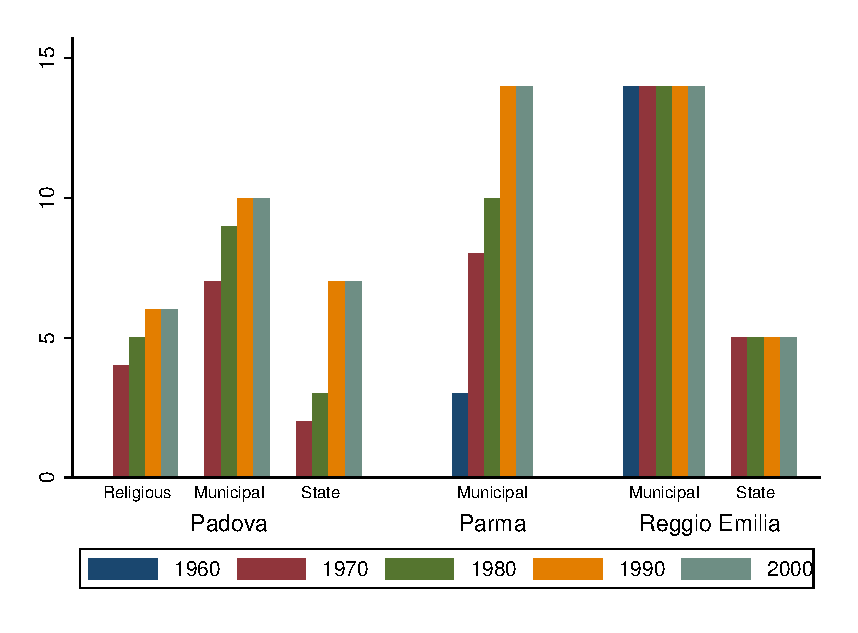
\includegraphics[scale=0.7]{../../output/aggregateAdministrative.eps}
\end{center}
\tiny{\textbf{Note:} The first three groups of bars correspond to Padova, the fourth group corresponds to Parma, and the last two groups correspond to Reggio Emilia.}
\end{frame}

\begin{frame}
\frametitle{Administrative Components}
\begin{center}
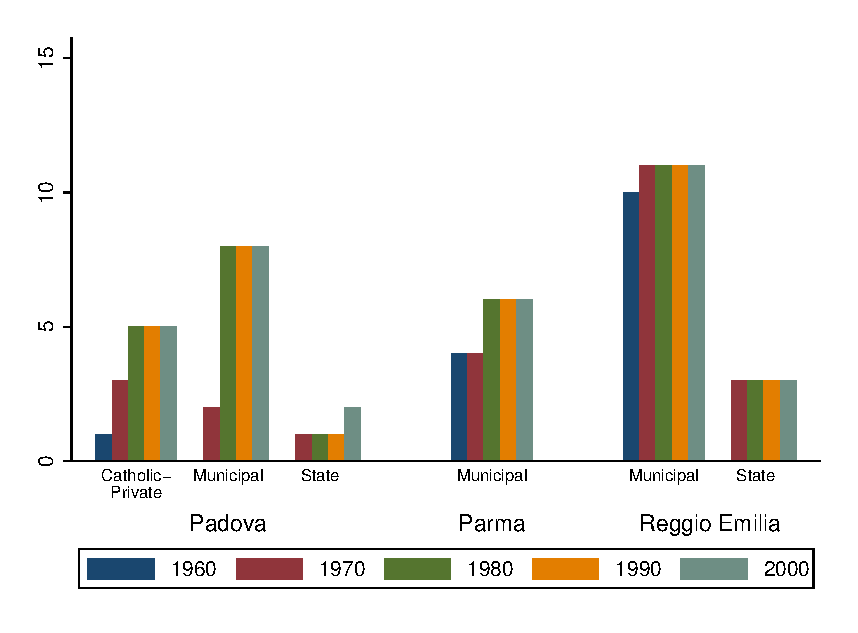
\includegraphics[scale=0.7]{../../output/aggregatePedagogical.eps}
\end{center}
\tiny{\textbf{Note:} The first three groups of bars correspond to Padova, the fourth group corresponds to Parma, and the last two groups correspond to Reggio Emilia.}
\end{frame}


% -------------------------------------------------------------------------------------------------

\begin{frame}
\frametitle{Summary of Responses}
\footnotesize
\begin{itemize}
	\item Hours of center-based care is one commonality largely shared by the surveyed programs
	\item  Teachers have dedicated work hours for professional development and documentation
	\item Municipal schools in the three cities shared priorities of enrolling disadvantaged children
	\item It was not until the 1980s that at least one other system had a full-time educative coordinator
	\item Some pedagogical components not in the Reggio Approach: (i) no religious education; (ii) no preset curriculum; and (iii) little influence of Montessori relative to the influence of Malaguzzi. 
	\item The presence of an arts specialist is more distinctive. Outside of the Reggio Approach, this has only been seen in Padova's municipal school since the 1980s. Although, visual arts were used in a preschool setting in all the other programs by the 1980s.  
\end{itemize}
\end{frame}

% -------------------------------------------------------------------------------------------------
\begin{frame}
\frametitle{Historical Records of Preschool Attendance}
\begin{itemize}
	\item We additionally unearthed paper records of preschool attendance in Reggio Emilia and Padova
	\item Attendance in both cities is close to 100\% 
\end{itemize}
\end{frame}

\begin{frame}
\frametitle{Number of Children Ages 3-5 Enrolled in Preschool, Reggio Emilia}
\begin{center}
\includegraphics[width=0.8\textwidth]{../../output/image/Enrollement_Preschool_RE.pdf}
\end{center}
\tiny{\textbf{Note:} The ``Enrolled in Pre-School" series is not defined for a specific age and could include children outside of the 3-5 range. Therefore, it is possible that the blue line could be greater than the red line at a particular point of time.}
\end{frame}

\begin{frame}
\frametitle{Number of Children Ages 3-5 Enrolled in Preschool, Padova}
\begin{center}
\includegraphics[scale=0.36]{../../output/image/Enrollement_Preschool_Padova.pdf}
\end{center}
\tiny{\textbf{Note:} A potential reason why there are more enrolled children than total number of children during some years is that the enrollment variable is not restricted to the 3-5 age range. We are further investigating the data sources to confirm that this is the reason that enrollment is greater that the total number of children for some years.}
\end{frame}

\begin{frame}
\frametitle{Percent of Children Ages 3-5 Enrolled in Preschool, Reggio Emilia and Padova}
\begin{center}
\includegraphics[scale=0.33]{../../output/image/Enrollement_Preschool_age3-5.pdf}
\end{center}
\tiny{\textbf{Note:} A potential reason why the rate of enrollment is greater than 1 for some years is that the enrollment variable is not restricted to the 3-5 age range. We are further investigating the data sources to confirm that this is the reason that enrollment is greater that the total number of children for some years.}
\end{frame}
% -------------------------------------------------------------------------------------------------

\begin{frame}
\frametitle{Methodology}
\begin{itemize}
	\item OLS with varying control sets 
	\item Difference-in-difference (DiD) across cities 
	\item AIPW to account for selection into the Reggio Approach beyond OLS and DiD
	\item Propensity score matching to further test for the presence of selection 
\end{itemize}
\end{frame}

% -------------------------------------------------------------------------------------------------

\begin{frame}
\frametitle{Summary of Results}
\begin{itemize}
	\item Children
	\begin{itemize}
		\item Improved non-cognitive outcome (SDQ)
	\end{itemize}
	\item Adolescents
	\begin{itemize}
		\item Improved non-cognitive and mental health outcomes, less likely to drop out of school, more likely to dislike school, more likely to be unhealthy (obese and less exercise)
	\end{itemize}
	\item Adults
		\begin{itemize}
		\item The most positive and significant results are seen when compared with adults who attended no preschool
		\item More likely to be employed (40s) and work more hours (30s and 40s)
		\item Less depressed and more internal locus of control (40s)
		\item More likely to vote (40s)
		\end{itemize}
\end{itemize}
\end{frame}

% -------------------------------------------------------------------------------------------------

\begin{frame}
\frametitle{Reggio Approach vs. Non-Reggio Approach, Child Cohort}
\centering
\adjustbox{max height=\dimexpr\textheight-5.5cm\relax,
           max width=\textwidth}{
\begin{tabular}{l c c c c c c}
\toprule
 & None & BIC & Full & AIPW & DidPm & DidPv \\
\midrule
IQ Score &     -0.02 &     -0.03 &     -0.03 &     -0.02 &      0.03 &     -0.01 \\
& (     0.02 ) & (     0.02 ) & (     0.02 ) & (     0.02 ) & (     0.04 ) & (     0.03 ) \\
& \textit{ 410 } & \textit{ 410 } & \textit{ 410 } & \textit{ 410 } & \textit{ 762 } & \textit{ 790 } \\
IQ Factor &     -0.07 &     -0.13 &     -0.12 &     -0.12 &      0.14 &      0.03 \\
& (     0.10 ) & (     0.10 ) & (     0.10 ) & (     0.10 ) & (     0.17 ) & (     0.15 ) \\
& \textit{ 410 } & \textit{ 410 } & \textit{ 410 } & \textit{ 410 } & \textit{ 762 } & \textit{ 790 } \\
SDQ Composite - Child & \textbf{      0.70 } & \textbf{      0.96 } & \textbf{      1.21 } & \textbf{     0.93} &      0.10 & \textbf{      1.18 } \\
& (     0.47 ) & (     0.46 ) & (     0.45 ) & (     0.46 ) & (     0.84 ) & (     0.75 ) \\
& \textit{ 409 } & \textit{ 409 } & \textit{ 409 } & \textit{ 409 } & \textit{ 761 } & \textit{ 789 } \\
Obese &     -0.00 &      0.04 &      0.03 &      0.05 &      0.03 &     -0.05 \\
& (     0.05 ) & (     0.05 ) & (     0.05 ) & (     0.04 ) & (     0.08 ) & (     0.07 ) \\
& \textit{ 410 } & \textit{ 410 } & \textit{ 410 } & \textit{ 410 } & \textit{ 762 } & \textit{ 790 } \\
Overweight & \textbf{      0.05 } &      0.03 &      0.05 &      0.03 &     -0.06 & \textbf{      0.09 } \\
& (     0.03 ) & (     0.03 ) & (     0.04 ) & (     0.03 ) & (     0.07 ) & (     0.05 ) \\
& \textit{ 410 } & \textit{ 410 } & \textit{ 410 } & \textit{ 410 } & \textit{ 762 } & \textit{ 790 } \\
Health is Good &     -0.05 &     -0.03 &     -0.01 &     -0.02 &      0.08 &     -0.05 \\
& (     0.05 ) & (     0.05 ) & (     0.05 ) & (     0.05 ) & (     0.09 ) & (     0.07 ) \\
& \textit{ 409 } & \textit{ 409 } & \textit{ 409 } & \textit{ 409 } & \textit{ 761 } & \textit{ 788 } \\
Not Excited to Learn &     -0.00 &      0.00 &     -0.00 &     -0.00 &      0.03 &     -0.03 \\
& (     0.02 ) & (     0.02 ) & (     0.02 ) & (     0.02 ) & (     0.04 ) & (     0.04 ) \\
& \textit{ 410 } & \textit{ 410 } & \textit{ 410 } & \textit{ 410 } & \textit{ 762 } & \textit{ 790 } \\
Problems Sitting Still &      0.02 &      0.03 &      0.00 &      0.02 &     -0.08 &     -0.04 \\
& (     0.03 ) & (     0.03 ) & (     0.03 ) & (     0.03 ) & (     0.07 ) & (     0.05 ) \\
& \textit{ 410 } & \textit{ 410 } & \textit{ 410 } & \textit{ 410 } & \textit{ 762 } & \textit{ 790 } \\
How Much Child Likes School &      0.02 &      0.00 &      0.04 &     -0.01 &      0.07 &      0.10 \\
& (     0.06 ) & (     0.06 ) & (     0.06 ) & (     0.06 ) & (     0.10 ) & (     0.09 ) \\
& \textit{ 408 } & \textit{ 408 } & \textit{ 408 } & \textit{ 408 } & \textit{ 758 } & \textit{ 788 } \\
\bottomrule
\end{tabular}
}
\end{frame}

\begin{frame}
\centering
\frametitle{Reggio Approach vs. Non-Reggio Approach, Adolescent Cohort}
\adjustbox{max height=\dimexpr\textheight-5.5cm\relax,
           max width=\textwidth}{
\begin{tabular}{l c c c c c c}
\toprule
 & None & Bic & Full & AIPW & DidPm & DidPv \\
\midrule
IQ Score &     -0.03 &     -0.04 &      0.00 &     -0.03 &     -0.04 &     -0.05 \\
& (     0.03 ) & (     0.03 ) & (     0.03 ) & (     0.04 ) & (     0.05 ) & (     0.05 ) \\
& \textit{ 286 } & \textit{ 286 } & \textit{ 286 } & \textit{ 286 } & \textit{ 530 } & \textit{ 561 } \\
IQ Factor &     -0.12 & \textbf{     -0.17 } &     -0.02 &     -0.13 &     -0.06 &     -0.20 \\
& (     0.10 ) & (     0.11 ) & (     0.11 ) & (     0.12 ) & (     0.17 ) & (     0.17 ) \\
& \textit{ 286 } & \textit{ 286 } & \textit{ 286 } & \textit{ 286 } & \textit{ 530 } & \textit{ 561 } \\
SDQ Composite - Child &     -0.03 &     -0.16 &      0.31 &      0.21 &      0.50 &     -0.60 \\
& (     0.59 ) & (     0.70 ) & (     0.62 ) & (     0.70 ) & (     1.09 ) & (     0.80 ) \\
& \textit{ 286 } & \textit{ 286 } & \textit{ 286 } & \textit{ 286 } & \textit{ 530 } & \textit{ 556 } \\
SDQ Composite &      0.89 &      0.90 &      0.69 &      0.45 & \textbf{      1.62 } &      0.68 \\
& (     0.63 ) & (     0.71 ) & (     0.72 ) & (     0.77 ) & (     1.06 ) & (     0.94 ) \\
& \textit{ 284 } & \textit{ 284 } & \textit{ 284 } & \textit{ 284 } & \textit{ 526 } & \textit{ 557 } \\
Depression Score - positive & \textbf{      1.38 } & \textbf{      1.75 } & \textbf{      1.71 } &      1.24 & \textbf{      3.14 } & \textbf{      1.86 } \\
& (     0.78 ) & (     0.88 ) & (     0.91 ) & (     0.93 ) & (     1.18 ) & (     1.14 ) \\
& \textit{ 279 } & \textit{ 279 } & \textit{ 279 } & \textit{ 279 } & \textit{ 512 } & \textit{ 550 } \\
Locus of Control - positive &      0.03 &      0.05 &      0.04 &     -0.01 & \textbf{     -0.25 } &      0.11 \\
& (     0.09 ) & (     0.10 ) & (     0.09 ) & (     0.10 ) & (     0.15 ) & (     0.13 ) \\
& \textit{ 283 } & \textit{ 283 } & \textit{ 283 } & \textit{ 283 } & \textit{ 522 } & \textit{ 556 } \\
Obese & \textbf{      0.08 } & \textbf{      0.11 } & \textbf{      0.09 } & \textbf{     0.10} &      0.00 &      0.09 \\
& (     0.04 ) & (     0.05 ) & (     0.04 ) & (     0.04 ) & (     0.07 ) & (     0.07 ) \\
& \textit{ 286 } & \textit{ 286 } & \textit{ 286 } & \textit{ 286 } & \textit{ 530 } & \textit{ 561 } \\
Overweight &     -0.01 &      0.00 &      0.00 &      0.01 &     -0.08 &      0.02 \\
& (     0.02 ) & (     0.03 ) & (     0.02 ) & (     0.03 ) & (     0.06 ) & (     0.03 ) \\
& \textit{ 286 } & \textit{ 286 } & \textit{ 286 } & \textit{ 286 } & \textit{ 530 } & \textit{ 561 } \\
Health is Good &      0.06 &      0.07 & \textbf{      0.09 } &      0.06 &      0.11 & \textbf{      0.13 } \\
& (     0.06 ) & (     0.06 ) & (     0.06 ) & (     0.07 ) & (     0.10 ) & (     0.09 ) \\
& \textit{ 285 } & \textit{ 285 } & \textit{ 285 } & \textit{ 285 } & \textit{ 529 } & \textit{ 560 } \\
Go To School &      0.03 &      0.01 &      0.03 &      0.01 &     -0.00 &      0.04 \\
& (     0.02 ) & (     0.02 ) & (     0.03 ) & (     0.02 ) & (     0.03 ) & (     0.03 ) \\
& \textit{ 286 } & \textit{ 286 } & \textit{ 286 } & \textit{ 286 } & \textit{ 530 } & \textit{ 561 } \\
How Much Child Likes School &     -0.12 &     -0.11 & \textbf{     -0.18 } &     -0.00 &      0.08 &     -0.12 \\
& (     0.11 ) & (     0.13 ) & (     0.12 ) & (     0.14 ) & (     0.19 ) & (     0.16 ) \\
& \textit{ 273 } & \textit{ 273 } & \textit{ 273 } & \textit{ 273 } & \textit{ 508 } & \textit{ 543 } \\
Days of Sport (Weekly) & \textbf{     -0.41 } & \textbf{     -0.43 } &     -0.29 &     -0.46 & \textbf{     -0.84 } &     -0.48 \\
& (     0.23 ) & (     0.26 ) & (     0.26 ) & (     0.26 ) & (     0.38 ) & (     0.34 ) \\
& \textit{ 280 } & \textit{ 280 } & \textit{ 280 } & \textit{ 280 } & \textit{ 516 } & \textit{ 536 } \\
\bottomrule
\end{tabular}
}
\end{frame}

\begin{frame}
\centering
\frametitle{Reggio Approach vs. Other Preschools, Adult Cohorts}
\adjustbox{max height=\dimexpr\textheight-5.5cm\relax,
           max width=\textwidth}{
\begin{tabular}{l c c c c c c c c c c}
\toprule
 & None30 & BIC30 & Full30 & DidPm30 & DidPv30 & AIPW30 & None40 & BIC40 & Full40 & AIPW40 \\
\midrule
Graduate from High School &     -0.04 &     -0.03 &     -0.05 & \textbf{     -0.17 } &      0.08 &     -0.06 & \textbf{      0.13 } &      0.09 & \textbf{      0.11 } &      0.01 \\
& (     0.05 ) & (     0.05 ) & (     0.05 ) & (     0.06 ) & (     0.06 ) & (     0.05 ) & (     0.07 ) & (     0.07 ) & (     0.07 ) & (     0.06 ) \\
& \textit{ 153 } & \textit{ 153 } & \textit{ 153 } & \textit{ 299 } & \textit{ 326 } & \textit{ 153 } & \textit{ 161 } & \textit{ 161 } & \textit{ 161 } & \textit{ 161 } \\
Max Edu: University &      0.04 &      0.04 &      0.03 & \textbf{     -0.18 } &     -0.17 &      0.02 &      0.08 &      0.05 &      0.03 &      0.05 \\
& (     0.07 ) & (     0.07 ) & (     0.07 ) & (     0.08 ) & (     0.12 ) & (     0.07 ) & (     0.06 ) & (     0.05 ) & (     0.05 ) & (     0.06 ) \\
& \textit{ 153 } & \textit{ 153 } & \textit{ 153 } & \textit{ 299 } & \textit{ 326 } & \textit{ 153 } & \textit{ 161 } & \textit{ 161 } & \textit{ 161 } & \textit{ 161 } \\
Employed &     -0.02 &     -0.02 &     -0.01 &     -0.03 &      0.02 &     -0.02 &      0.01 &      0.01 &      0.01 &      0.02 \\
& (     0.03 ) & (     0.04 ) & (     0.04 ) & (     0.06 ) & (     0.08 ) & (     0.03 ) & (     0.03 ) & (     0.03 ) & (     0.04 ) & (     0.03 ) \\
& \textit{ 153 } & \textit{ 153 } & \textit{ 153 } & \textit{ 299 } & \textit{ 326 } & \textit{ 153 } & \textit{ 161 } & \textit{ 161 } & \textit{ 161 } & \textit{ 161 } \\
Hours Worked Per Week &      1.13 &      0.40 &      1.22 &      0.16 &     -0.12 &      0.53 &     -0.86 &     -0.98 &     -1.25 &     -0.10 \\
& (     1.90 ) & (     2.04 ) & (     2.08 ) & (     2.87 ) & (     3.44 ) & (     2.43 ) & (     1.90 ) & (     2.03 ) & (     2.14 ) & (     1.89 ) \\
& \textit{ 123 } & \textit{ 123 } & \textit{ 123 } & \textit{ 266 } & \textit{ 292 } & \textit{ 123 } & \textit{ 146 } & \textit{ 146 } & \textit{ 146 } & \textit{ 146 } \\
Married or Cohabitating &      0.08 &      0.04 &      0.04 &     -0.01 &     -0.14 &      0.02 &      0.02 &      0.01 &      0.01 &      0.00 \\
& (     0.08 ) & (     0.08 ) & (     0.08 ) & (     0.08 ) & (     0.12 ) & (     0.08 ) & (     0.07 ) & (     0.07 ) & (     0.07 ) & (     0.07 ) \\
& \textit{ 153 } & \textit{ 153 } & \textit{ 153 } & \textit{ 299 } & \textit{ 326 } & \textit{ 153 } & \textit{ 161 } & \textit{ 161 } & \textit{ 161 } & \textit{ 161 } \\
Obese &     -0.02 &      0.04 &      0.00 &     -0.08 &     -0.04 &      0.02 &      0.03 &     -0.01 &     -0.04 &     -0.05 \\
& (     0.07 ) & (     0.06 ) & (     0.06 ) & (     0.07 ) & (     0.10 ) & (     0.06 ) & (     0.07 ) & (     0.07 ) & (     0.07 ) & (     0.09 ) \\
& \textit{ 153 } & \textit{ 153 } & \textit{ 153 } & \textit{ 299 } & \textit{ 326 } & \textit{ 153 } & \textit{ 161 } & \textit{ 161 } & \textit{ 161 } & \textit{ 161 } \\
Overweight &      0.04 &     -0.01 &     -0.01 & \textbf{      0.14 } &     -0.02 &     -0.01 &     -0.04 &     -0.03 &     -0.02 &      0.05 \\
& (     0.07 ) & (     0.06 ) & (     0.06 ) & (     0.08 ) & (     0.09 ) & (     0.07 ) & (     0.07 ) & (     0.07 ) & (     0.07 ) & (     0.07 ) \\
& \textit{ 153 } & \textit{ 153 } & \textit{ 153 } & \textit{ 299 } & \textit{ 326 } & \textit{ 153 } & \textit{ 161 } & \textit{ 161 } & \textit{ 161 } & \textit{ 161 } \\
Locus of Control - positive &      0.11 &      0.04 &      0.06 &      0.14 &     -0.19 &      0.04 &      0.13 &      0.14 &      0.11 &      0.08 \\
& (     0.12 ) & (     0.11 ) & (     0.12 ) & (     0.19 ) & (     0.19 ) & (     0.11 ) & (     0.13 ) & (     0.14 ) & (     0.14 ) & (     0.14 ) \\
& \textit{ 149 } & \textit{ 149 } & \textit{ 149 } & \textit{ 286 } & \textit{ 315 } & \textit{ 149 } & \textit{ 158 } & \textit{ 158 } & \textit{ 158 } & \textit{ 158 } \\
Depression Score - positive &      0.46 &     -0.53 &     -0.24 &     -0.39 &     -0.72 &     -0.63 &      0.57 & \textbf{      1.34 } &      0.99 &      0.99 \\
& (     1.05 ) & (     0.69 ) & (     0.67 ) & (     1.04 ) & (     1.52 ) & (     0.63 ) & (     0.91 ) & (     0.85 ) & (     0.89 ) & (     0.93 ) \\
& \textit{ 151 } & \textit{ 151 } & \textit{ 151 } & \textit{ 297 } & \textit{ 321 } & \textit{ 151 } & \textit{ 158 } & \textit{ 158 } & \textit{ 158 } & \textit{ 158 } \\
Ever Voted for Municipal &      0.02 &      0.00 &      0.01 &     -0.07 & \textbf{     -0.27 } &      0.01 &     -0.05 &      0.08 &      0.07 & \textbf{     0.10} \\
& (     0.08 ) & (     0.06 ) & (     0.07 ) & (     0.05 ) & (     0.09 ) & (     0.06 ) & (     0.08 ) & (     0.07 ) & (     0.07 ) & (     0.07 ) \\
& \textit{ 151 } & \textit{ 151 } & \textit{ 151 } & \textit{ 295 } & \textit{ 314 } & \textit{ 151 } & \textit{ 153 } & \textit{ 153 } & \textit{ 153 } & \textit{ 153 } \\
Ever Voted for Regional &     -0.01 &     -0.04 &     -0.03 &     -0.07 & \textbf{     -0.37 } &     -0.04 &     -0.03 &      0.09 &      0.08 & \textbf{     0.11} \\
& (     0.08 ) & (     0.07 ) & (     0.07 ) & (     0.05 ) & (     0.09 ) & (     0.06 ) & (     0.08 ) & (     0.07 ) & (     0.07 ) & (     0.08 ) \\
& \textit{ 151 } & \textit{ 151 } & \textit{ 151 } & \textit{ 295 } & \textit{ 314 } & \textit{ 151 } & \textit{ 153 } & \textit{ 153 } & \textit{ 153 } & \textit{ 153 } \\
\bottomrule
\end{tabular}
}
\end{frame}

\begin{frame}
\centering
\frametitle{Reggio Approach vs. No Preschool, Adult Cohorts}
\adjustbox{max height=\dimexpr\textheight-5.5cm\relax,
           max width=\textwidth}{
\begin{tabular}{l c c c c c c c c c c}
\toprule
 & None30 & BIC30 & Full30 & DidPm30 & DidPv30 & AIPW30 & None40 & BIC40 & Full40 & AIPW40 \\
\midrule
Graduate from High School &     -0.02 &      0.05 &      0.05 & \textbf{     -0.17 } &      0.06 &      0.06 &     -0.07 &     -0.01 &     -0.06 &     -0.01 \\
& (     0.05 ) & (     0.05 ) & (     0.05 ) & (     0.08 ) & (     0.07 ) & (     0.06 ) & (     0.05 ) & (     0.05 ) & (     0.06 ) & (     0.06 ) \\
& \textit{ 151 } & \textit{ 151 } & \textit{ 151 } & \textit{ 232 } & \textit{ 217 } & \textit{ 151 } & \textit{ 170 } & \textit{ 170 } & \textit{ 170 } & \textit{ 170 } \\
Max Edu: University &     -0.06 &      0.00 &     -0.01 & \textbf{     -0.17 } &      0.10 &      0.01 &      0.01 &      0.06 & \textbf{      0.11 } &      0.06 \\
& (     0.07 ) & (     0.08 ) & (     0.08 ) & (     0.09 ) & (     0.13 ) & (     0.07 ) & (     0.06 ) & (     0.06 ) & (     0.06 ) & (     0.06 ) \\
& \textit{ 151 } & \textit{ 151 } & \textit{ 151 } & \textit{ 232 } & \textit{ 217 } & \textit{ 151 } & \textit{ 170 } & \textit{ 170 } & \textit{ 170 } & \textit{ 170 } \\
Employed &      0.05 &      0.03 &      0.06 &     -0.04 &     -0.00 &      0.02 & \textbf{      0.06 } & \textbf{      0.08 } &      0.05 & \textbf{     0.08} \\
& (     0.05 ) & (     0.05 ) & (     0.04 ) & (     0.07 ) & (     0.09 ) & (     0.04 ) & (     0.04 ) & (     0.03 ) & (     0.03 ) & (     0.05 ) \\
& \textit{ 151 } & \textit{ 151 } & \textit{ 151 } & \textit{ 232 } & \textit{ 217 } & \textit{ 151 } & \textit{ 169 } & \textit{ 169 } & \textit{ 169 } & \textit{ 169 } \\
Hours Worked Per Week & \textbf{      7.93 } & \textbf{      5.10 } & \textbf{      6.27 } &     -1.18 &     -0.35 &      4.28 & \textbf{      5.71 } & \textbf{      7.29 } & \textbf{      7.39 } & \textbf{     7.24} \\
& (     2.74 ) & (     3.00 ) & (     2.90 ) & (     3.19 ) & (     3.90 ) & (     3.03 ) & (     2.42 ) & (     2.39 ) & (     2.60 ) & (     2.23 ) \\
& \textit{ 124 } & \textit{ 124 } & \textit{ 124 } & \textit{ 205 } & \textit{ 190 } & \textit{ 124 } & \textit{ 151 } & \textit{ 151 } & \textit{ 151 } & \textit{ 151 } \\
Married or Cohabitating &      0.00 &     -0.09 &     -0.10 &      0.04 &     -0.04 &     -0.08 &      0.02 &      0.01 &      0.05 &      0.04 \\
& (     0.08 ) & (     0.08 ) & (     0.09 ) & (     0.11 ) & (     0.14 ) & (     0.08 ) & (     0.07 ) & (     0.07 ) & (     0.08 ) & (     0.08 ) \\
& \textit{ 151 } & \textit{ 151 } & \textit{ 151 } & \textit{ 232 } & \textit{ 217 } & \textit{ 151 } & \textit{ 170 } & \textit{ 170 } & \textit{ 170 } & \textit{ 170 } \\
Obese &     -0.01 & \textbf{      0.10 } & \textbf{      0.10 } &      0.02 & \textbf{     -0.23 } & \textbf{     0.10} & \textbf{     -0.14 } &     -0.08 &     -0.01 &     -0.07 \\
& (     0.07 ) & (     0.06 ) & (     0.07 ) & (     0.08 ) & (     0.12 ) & (     0.06 ) & (     0.07 ) & (     0.08 ) & (     0.08 ) & (     0.08 ) \\
& \textit{ 151 } & \textit{ 151 } & \textit{ 151 } & \textit{ 232 } & \textit{ 217 } & \textit{ 151 } & \textit{ 170 } & \textit{ 170 } & \textit{ 170 } & \textit{ 170 } \\
Overweight &      0.05 &     -0.04 &     -0.01 &      0.06 &      0.01 &     -0.03 &      0.03 &     -0.04 &     -0.07 &     -0.06 \\
& (     0.07 ) & (     0.06 ) & (     0.06 ) & (     0.10 ) & (     0.10 ) & (     0.06 ) & (     0.07 ) & (     0.07 ) & (     0.07 ) & (     0.08 ) \\
& \textit{ 151 } & \textit{ 151 } & \textit{ 151 } & \textit{ 232 } & \textit{ 217 } & \textit{ 151 } & \textit{ 170 } & \textit{ 170 } & \textit{ 170 } & \textit{ 170 } \\
Locus of Control - positive &      0.08 &     -0.10 &     -0.11 & \textbf{      0.46 } &     -0.03 &     -0.09 &      0.14 & \textbf{      0.20 } & \textbf{      0.28 } & \textbf{     0.27} \\
& (     0.14 ) & (     0.13 ) & (     0.13 ) & (     0.22 ) & (     0.22 ) & (     0.15 ) & (     0.13 ) & (     0.13 ) & (     0.14 ) & (     0.14 ) \\
& \textit{ 148 } & \textit{ 148 } & \textit{ 148 } & \textit{ 221 } & \textit{ 206 } & \textit{ 148 } & \textit{ 165 } & \textit{ 165 } & \textit{ 165 } & \textit{ 165 } \\
Depression Score - positive & \textbf{      1.57 } &     -0.34 &     -0.35 &     -0.67 &      1.02 &     -0.22 & \textbf{      2.25 } & \textbf{      2.23 } & \textbf{      2.10 } & \textbf{     2.47} \\
& (     1.01 ) & (     0.88 ) & (     0.91 ) & (     1.25 ) & (     1.74 ) & (     0.86 ) & (     0.92 ) & (     0.95 ) & (     1.07 ) & (     1.15 ) \\
& \textit{ 149 } & \textit{ 149 } & \textit{ 149 } & \textit{ 230 } & \textit{ 214 } & \textit{ 149 } & \textit{ 168 } & \textit{ 168 } & \textit{ 168 } & \textit{ 168 } \\
Ever Voted for Municipal & \textbf{      0.19 } &      0.07 &      0.07 &      0.02 &      0.06 &      0.06 & \textbf{      0.19 } & \textbf{      0.12 } &      0.11 & \textbf{     0.14} \\
& (     0.08 ) & (     0.07 ) & (     0.07 ) & (     0.06 ) & (     0.11 ) & (     0.08 ) & (     0.08 ) & (     0.08 ) & (     0.08 ) & (     0.07 ) \\
& \textit{ 148 } & \textit{ 148 } & \textit{ 148 } & \textit{ 228 } & \textit{ 207 } & \textit{ 148 } & \textit{ 153 } & \textit{ 153 } & \textit{ 153 } & \textit{ 153 } \\
Ever Voted for Regional & \textbf{      0.14 } &      0.02 &      0.03 &      0.01 &     -0.07 &      0.02 & \textbf{      0.20 } & \textbf{      0.14 } & \textbf{      0.13 } & \textbf{     0.16} \\
& (     0.08 ) & (     0.07 ) & (     0.07 ) & (     0.06 ) & (     0.10 ) & (     0.08 ) & (     0.08 ) & (     0.08 ) & (     0.08 ) & (     0.09 ) \\
& \textit{ 148 } & \textit{ 148 } & \textit{ 148 } & \textit{ 228 } & \textit{ 207 } & \textit{ 148 } & \textit{ 153 } & \textit{ 153 } & \textit{ 153 } & \textit{ 153 } \\
\bottomrule
\end{tabular}
}
\end{frame}


%%
%%--------------------------- Content ends here ---------------------------------------------------
%%

% --------------------- Bibliography hidden with a save box ---------------------------------------
\mode<all>
\bibliographystyle{chicago}
\savebox\hiddenbib{\parbox{\textwidth}{\bibliography{heckman}}}

\end{document} 